\section{\computerrl 框架}\label{sec:framework}
GUI 面向人类的设计会阻碍智能体效率，而环境可扩展性有限又制约了大规模训练。
本节介绍 \computerrl 框架（见图~\ref{figs:framework}）。该框架采用 API-GUI 范式，将类人的 GUI 交互与高效 API 调用相结合。此外，我们开发了一个可扩展、可并行运行的 Ubuntu 桌面环境，并采用全异步 RL 框架来实现高效训练。

\begin{figure}[t!]
    \centering
    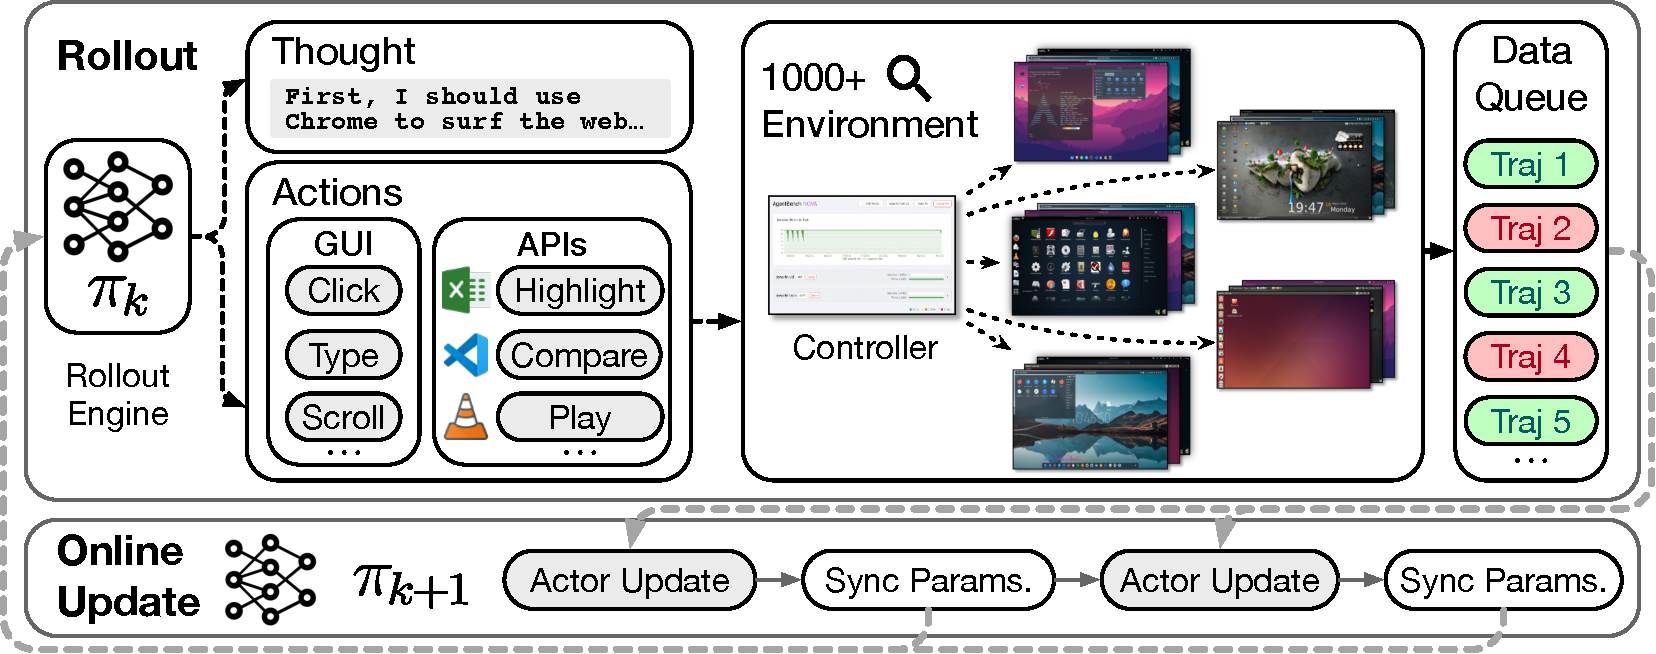
\includegraphics[width=0.95\textwidth]{images/framework.pdf}
    \caption{\computerrl 框架概览。我们提出一种 API-GUI 动作范式，将自动构建的 API 与 GUI 动作无缝结合，以提高智能体的效率与有效性。包含 1,000 多个真实实例的大规模并行桌面环境与异步 RL 框架相结合，可实现高效采样与稳健的智能体训练。}
    \label{figs:framework}
    \vspace{-3mm}
\end{figure}

\subsection{通用 API-GUI 范式}\label{sec:hybrid-action-space}
现有 GUI 智能体由于依赖类人交互而面临挑战；基于 API 的控制虽然高效，却会引入实现复杂性与安全限制。为解决这些问题，我们提出 API-GUI 范式，将两类动作空间统一起来，使智能体既能利用 API 的效率，又能保留 GUI 的通用性。

我们开发了一套基于 LLM 的应用程序 API 自动开发工作流~\citep{yang2024swe,wang2024openhands}，显著降低了创建 API 的门槛。用户提供示例任务，系统则通过以下三个阶段自主生成 API 代码与测试用例：
\begin{itemize}[leftmargin=1.5em,itemsep=0pt,parsep=0.2em,topsep=0.0em,partopsep=0.0em]
    \item \textbf{需求分析：}用户为目标应用程序提供任务示例。我们的 LLM 分析这些实例，提取必要功能，并与现有 API 接口对比以识别缺口。系统会为尚未覆盖的功能自动生成新接口，并优先设计通用函数，以降低复杂度并增强易用性。

    \item \textbf{API 实现：}该工作流逐个遍历接口定义，使用指定的 Python 库实现 API 功能。系统还会实现错误处理机制与日志记录，以便调试和维护。

    \item \textbf{测试用例生成：}与 \citet{li2024largelanguagemodelstest} 类似，我们从两方面验证 API 的正确性：(1) 调用时不存在运行时错误；(2) 在不同参数输入下返回正确结果。失败的 API 会接收错误反馈并进行自主修正。
\end{itemize}

该方法只需极少的人工干预即可创建面向特定应用程序的 API。我们已经为多个 Ubuntu 应用程序开发了 API 集，并通过实验验证了其有效性。详细的 API 开发工作流见附录~\ref{apdx:api_construction}。
智能体动作空间与提示词设计分别详见附录~\ref{apdx:action_space}和~\ref{apdx:agent_prompt}。

\subsection{面向大规模并行的稳定 Ubuntu 环境}\label{sec:stable-ubuntu}
稳定且可扩展的 Ubuntu 环境，是构建行为克隆数据并开展大规模 RL 训练的必要条件。在 OSWorld~\citep{xie2024osworld} 基础上，我们识别出以下关键局限：

\begin{itemize}[leftmargin=1.5em,itemsep=0pt,parsep=0.2em,topsep=0.0em,partopsep=0.0em]
    \item \textbf{资源密集与稳定性问题：}虚拟机大量占用 CPU，并且在高并发下不稳定，会造成性能下降与系统卡死。
    \item \textbf{网络瓶颈：}繁重工作负载会带来网络开销、连接失败与 IP 地址丢失，妨碍智能体交互和日志记录。
    \item \textbf{缺少原生分布式支持：}OSWorld 不支持多节点集群，因而无法高效进行分布式部署。
\end{itemize}

为解决这些局限，我们构建了一套稳健且可并行化的 OSWorld 基础设施（见图~\ref{figs:framework}），包含以下创新：
\begin{itemize}[leftmargin=1.5em,itemsep=0pt,parsep=0.2em,topsep=0.0em,partopsep=0.0em]
    \item \textbf{标准化的解耦接口：}我们通过 AgentBench API 重构环境，提供统一接口，将环境执行与计算后端解耦，并支持灵活的资源管理。
    \item \textbf{轻量级虚拟机部署：}我们使用 \href{https://github.com/qemus/qemu}{\texttt{qemu-in-dockere}} 部署容器化 Ubuntu 虚拟机；精简后的镜像减少了网络问题并优化资源使用，显著降低每个实例的 CPU 消耗。
    \item \textbf{分布式多节点集群：}我们采用\href{https://github.com/grpc}{基于 gRPC 的}通信，将多个 CPU 节点连接为分布式集群，并集中完成资源分配与编排。
    \item \textbf{基于 Web 的可视化与监控：}Web 界面可实时展示环境状态、智能体状态和资源分配情况，从而提升易用性与调试能力。
\end{itemize}

凭借这些技术改进，我们的系统能够在多节点 CPU 集群上部署\textbf{数千个}并发环境，这一点已经得到大量实证评估的验证。结果证实，我们的平台具有出色的稳定性、资源效率与可扩展性，可作为大规模 RL 与智能体研究的基础设施。

\subsection{用于高效训练的全异步 RL 框架}\label{sec:full-asynchronous}
现有 RL 框架依赖同步训练范式，交替进行轨迹采集与参数更新，导致训练效率低下。为解决这一局限，我们使用 AgentRL 框架~\citep{zhang2025model}开展全异步 RL 训练，并采用以下设计：

\begin{itemize}[leftmargin=1.5em,itemsep=0pt,parsep=0.2em,topsep=0.0em,partopsep=0.0em]
    \item \textbf{资源分区：}数据采集在专用资源上运行，训练器则从回放引擎以流式方式获取数据，从而避免二者相互阻塞。
    \item \textbf{动态批大小：}训练器以灵活的批大小处理传入数据，减少空闲时间并提高效率。
    \item \textbf{模块化组件隔离：}Actor、参考模型和 Critic 模块分别在专用资源上独立运行。我们使用 PyTorch 分布式进程组与 NCCL 高效共享参数。
    \item \textbf{缓解离策略偏差：}我们限制回放缓冲区大小，并在每次更新后同步轨迹，确保轨迹与最新策略保持接近。
\end{itemize}

通过稳定的高并发桌面环境，以及将训练与 rollout 解耦，我们显著提高了采样和 RL 训练效率。系统实现了较高的单 GPU 平均功耗，反映出较优的资源利用率。该设计通过动态平衡工作负载来支持可扩展、高吞吐的 RL 训练，从而显著提升硬件效率与整体训练吞吐量。
